%% content.tex
%%

%% ===========================
\chapter{Zusammenfassung}
%% ===========================

...

%% ===========================
\section{Ergebnisanalyse}
%% ===========================

Einer der wichtigsten Anforderungen ist die geringe Abfragegeschwindigkeit. Tabelle \ref{table:vergleich_abfragegeschwindigkeit} zeigt, dass man dieser Forderung gerecht wird. Ebenfalls deutlich zu erkennen, ist die Auswirkung des geänderten Schemas. Der Sprung von 98.000 ms auf 350 ms, ist durch die Reduktion zu erklären. Im neuen Schema existieren weniger Tabellen und weniger Tupeln. Außerdem ist im neuen Schema kein Verbund mehr notwendig, der sehr rechenintensiv sein kann. Allerdings muss einem klar sein, dass solche Maßnahmen, wie sie im Schemadesign ergriffen wurden, weitreichende Folgen haben. Eine davon ist eine sehr schlechte Erweiterbarkeit des Schemas. Im momentanen Schema können lediglich Spalten hinzugezogen werden, dessen Inhalt in allen Merkmalen vorhanden ist. Außerdem würde für jede Spalte weitere 18 Mio. Werte hinzukommen. Hinzunahme von Merkmal spezifischen Attributen führt ebenfalls zu hohem Änderungsaufwand. Die Konsequenz wäre eine Normalisierung die aus der data-Tabelle mehrere Tabellen macht. Dies würde den Einsatz von Verbundoperatoren erfordern. Dadurch würde die Abfragezeit wieder steigen. Allerdings wären wesentlich weniger Verbundoperatoren nötig als im alten Schema. Aufgrund dessen ist trotzdem mit einer deutlichen geringeren Abfragegeschwindigkeit zu rechnen.  

\begin{table}[htbp]
\centering
\label{table:vergleich_abfragegeschwindigkeit}
\begin{tabular} {l | r}
Versuchskomponente & Zeit in ms  \\ \hline
MSSQL Datenbank \& Altes Schema & 98000 \\
MSSQL Datenbank \& Neues Schema & 350 \\
H2 Datenbank \& Neues Schema & 80 \\
\end{tabular}
\caption{Abfragegeschwindigkeit Vergleich}
\end{table}

Bei Änderungen, die eine Steigerung der Komplexität mit sich bringen, stellt sich eine Frage. Ist die Datenbank nur aufgrund des geänderten Schemas deutlich schneller? Um dieser Frage nachzugehen wurden einige Tests durchgeführt. Abbildung \ref{ergebniss_vergleich} zeigt die Ergebnisse dieser Testreihen. Alle Test wurden auf einem Rechner durchgeführt. Dieser simulierte den Zugriff von 100 gleichzeitigen Benutzern, mithilfe von Multithreading. Die in den Diagrammen angegebene Zeit bezieht sich somit auf die Ausführung aller 100 Abfragen. Jeder simulierte Benutzer führt somit die auf der y Achse angegebene Anweisung aus. Beim obersten Balken in (a) sind es beispielsweise 15 Mio. SELECT-Anweisungen pro Benutzer. In (b) sind es hingegen 15 Mio. Update-Anweisungen. Die Insert-Anweisungen zeigt (c).    

\begin{figure}[htbp]
\centering
\subfigure[Vergleich anhand Select-Performance]{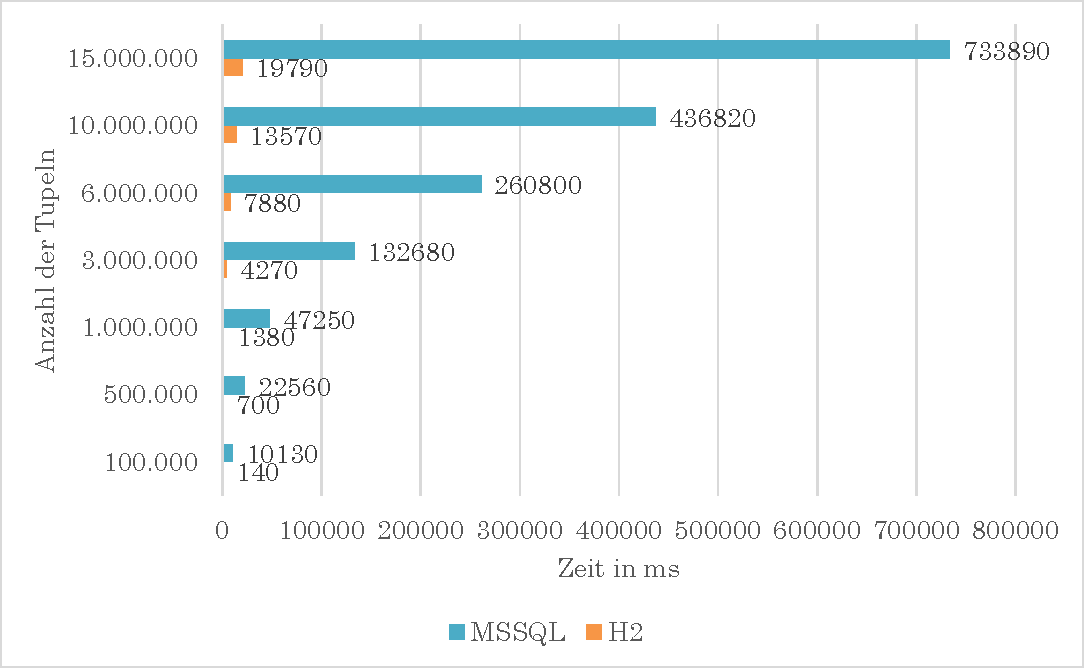
\includegraphics[width=0.49\textwidth]{charts/select.pdf}}\hfill
\subfigure[Vergleich anhand Update-Performance]{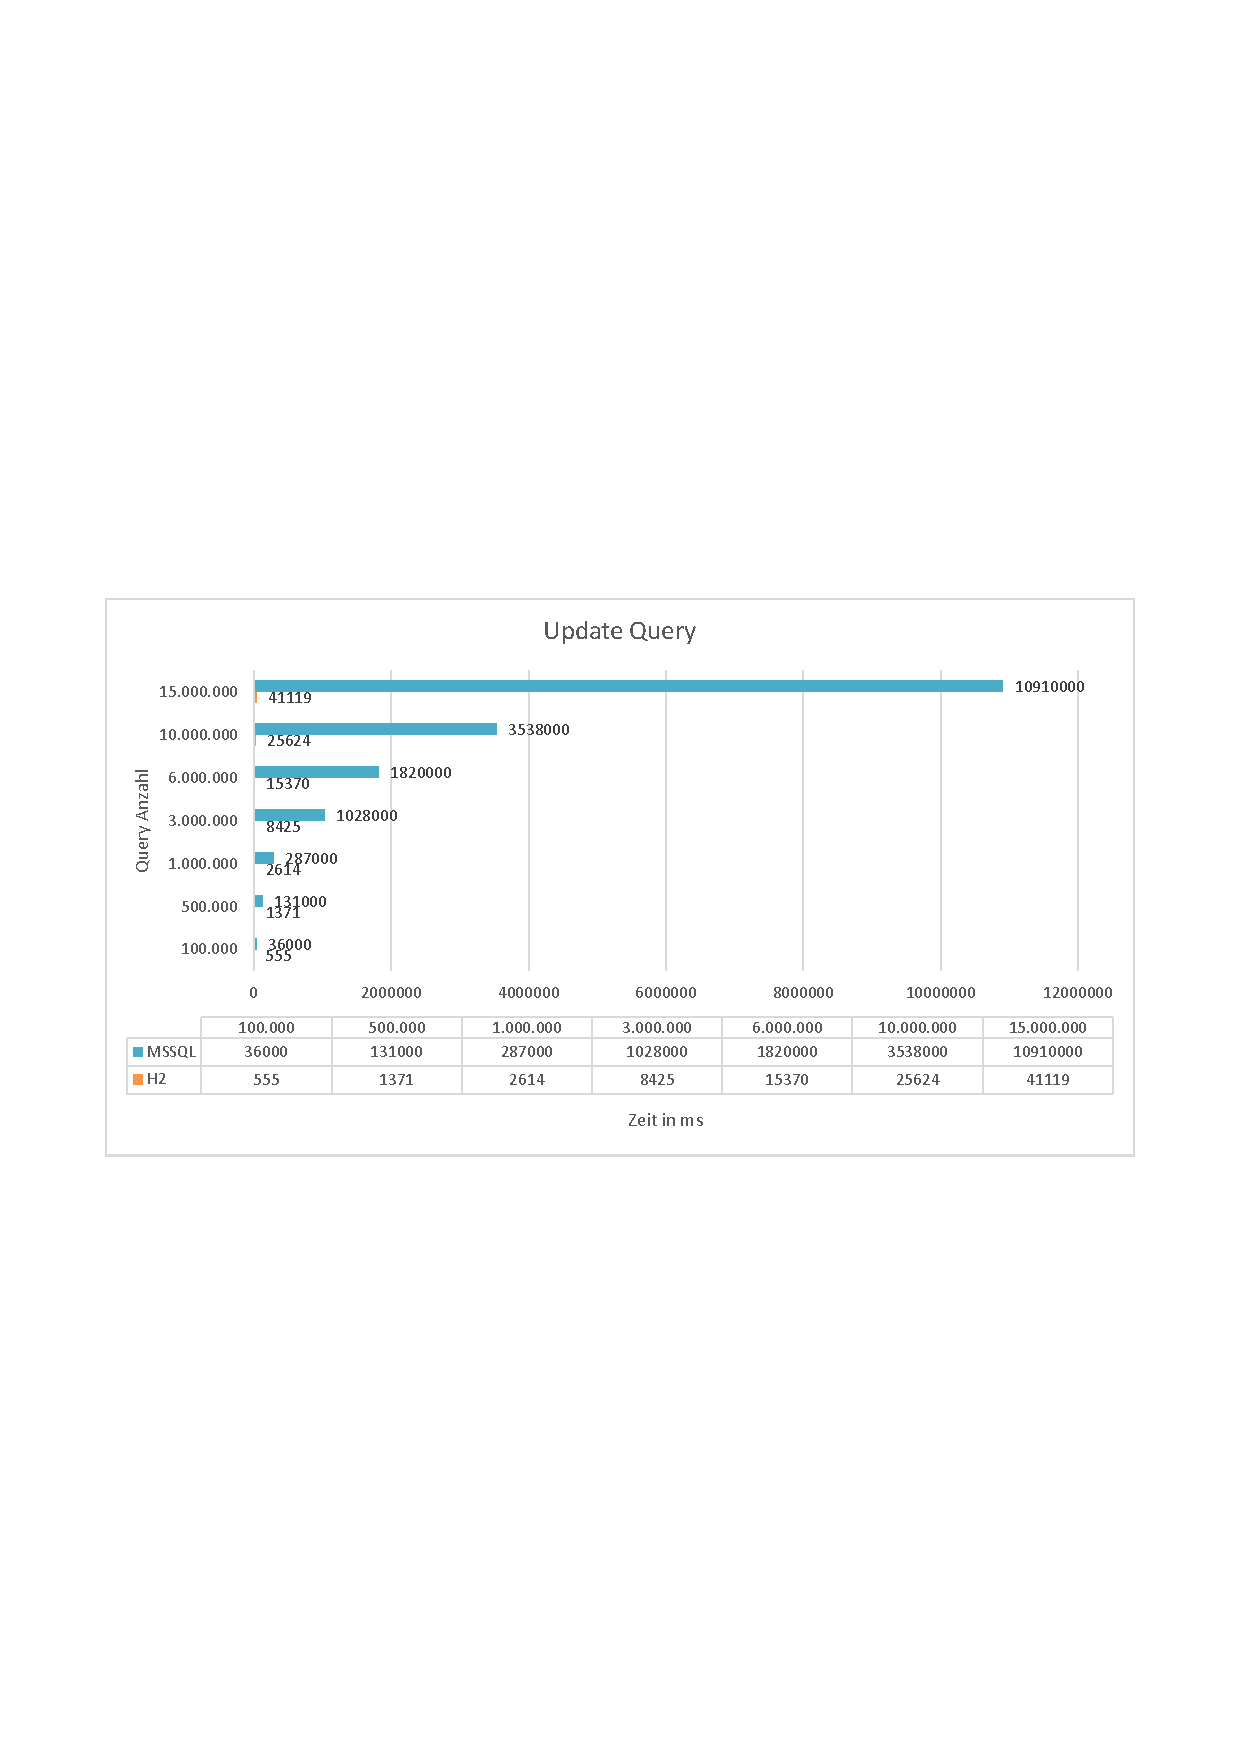
\includegraphics[width=0.49\textwidth]{charts/update.pdf}}\hfill
\subfigure[Vergleich anhand Insert-Performance]{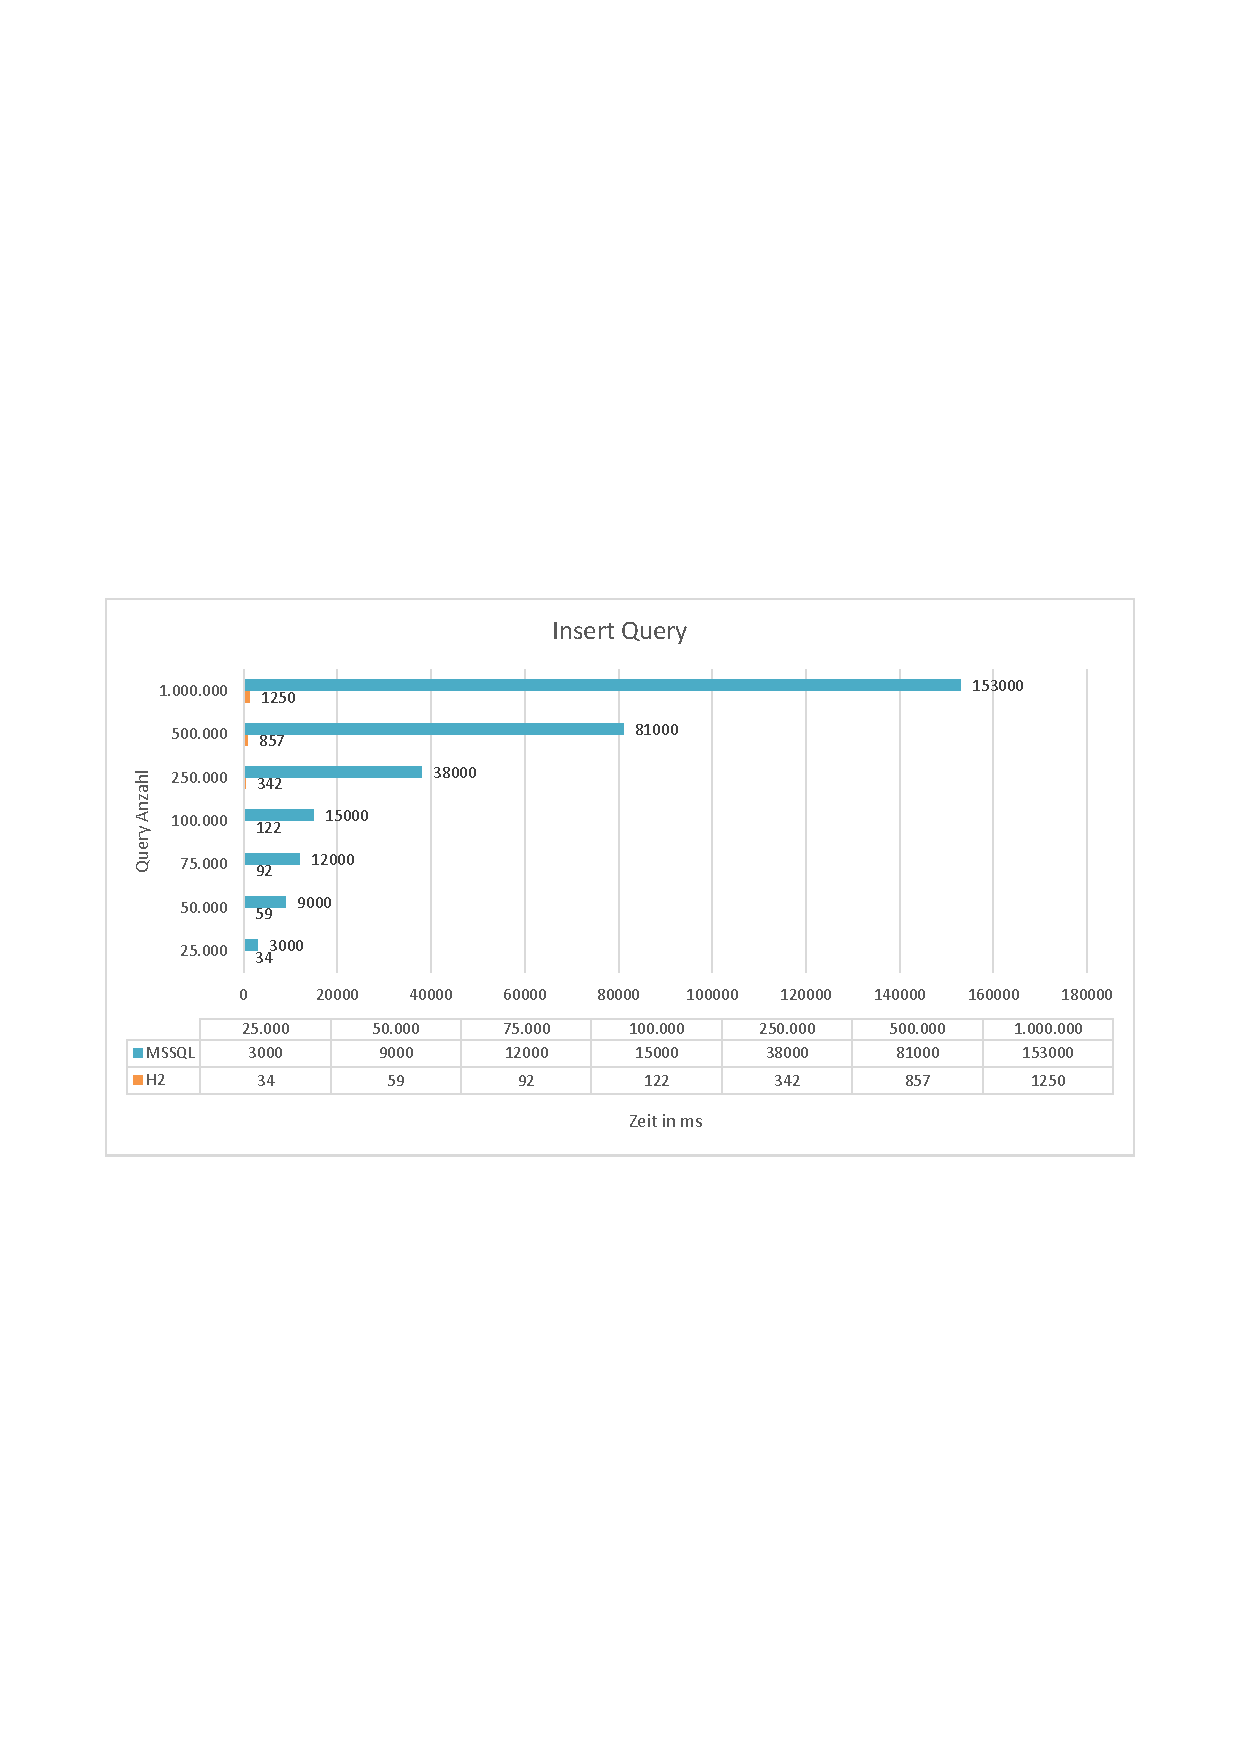
\includegraphics[width=0.5\textwidth]{charts/insert.pdf}}
\caption{Abfragegeschwindigkeit Vergleich}
\label{ergebniss_vergleich}
\end{figure}

Die Ergebnisse der Tests zeigen, dass die H2-Datenbank deutlich schneller ist als die MSSQL Datenbank. Der H2 ist bei SELECT-Anweisungen, um den Faktor 37 schneller. Bei Update-Anweisungen sogar um den Faktor 117 schneller. Ebenso bei Insert-Anweisungen, die einen Unterschied um den Faktor 124 aufweisen. Darauf lässt sich schließen, dass die H2-Datenbank mit ihren In-Memory-Tabellen deutlich schneller ist. Diese Geschwindigkeit wird durch den Verzicht auf Persistenz erlangt. In analytischen Systemen wo fast nur Leseoperationen durchgeführt werden stellt die mangelnde Persistenz kein großes Defizit dar. 

%% ===========================
\section{Handlungsempfehlungen}
%% ===========================

Desweiteren soll dargelegt werden, welche Möglichkeiten sich bei der Weiterführung des Projektes bieten und welche Schwierigkeiten auftreten könnten. 

Das momentane System ermittelt die Personen, die den stärksten Zusammenhang zueinander aufweisen, aufgrund der Anzahl der Verbindungen zwischen ihnen. Dabei wird lediglich die Häufigkeit gewertet. Um die stärke einer Beziehung zu bewerten könnten zusätzliche Regeln eingeführt werden. Diese Regeln müssten auf psychologischen Erkenntnissen und Erfahrungswerten aufbauen. Durch Regeln könnte die Aussagekraft des Ergebnisses weiter steigen. 

%% ===========================
\section{Ergebnis}
%% ===========================

...

%% ===========================
\section{Ausblick}
%% ===========================

...